\subsection{Proof of Relay}
\label{sec:proofofrelay}

HOPR incentivizes packet transformation and delivery using a mechanism called \textbf{proof of relay}. This mechanism guarantees that a node's relay services are verifiable.

Each node derives two keys, $s_i^{own}$ and $_i^{ack}$, by using the $s_i$ as given by the SPHINX packet, see section \href{appendix:keyderivation}{key derivation} for more details. $s_i^{own}$ and $s_{i+1}^{ack}$ serve as key shares of a 2-out-of-2 secret sharing between a node $n_i$ and the next downstream node $n_{i+1}$ along the chosen path. Once a node knows \textit{both} key shares, $s_i^{own}$ and $s_{i+1}^{ack}$, it is able to reconstruct $s_i^{response}$ to redeem the received ticket on-chain.

Whilst $s_i^{own}$ is derivable upon reception of a packet, $s_{i+1}^{ack}$ requires the cooperation of the next downstream node $n_{i+1}$ and is sent as an \textit{acknowledgement} if $n_{i+1}$ has received the transformed packet \textit{and} considers packet and the embedded ticket valid.

\begin{figure}[H]
    \centering
    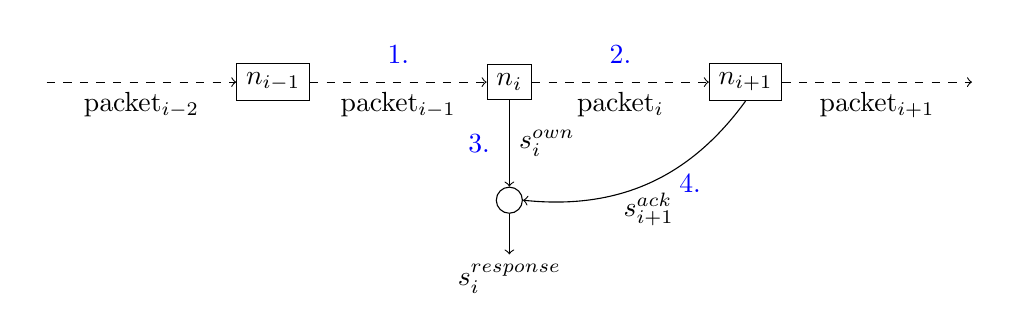
\begin{tikzpicture}[auto]
        \draw (0,0) node (a) {};
        \draw (3.0,0) node (b) [rectangle,draw] {$n_{i-1}$};
        \draw (6,0) node (c) [rectangle,draw] {$n_i$};
        \draw (9.0,0) node (d) [rectangle,draw] {$n_{i+1}$};
        \draw (12.0,0) node (e) {};

        \draw (6.0, -1.5) node [circle,draw] (intermediateResult) {};
        \draw (6.0, -2.5) node (response) {$s_i^{response}$};

        \draw [->,draw,dashed] (a.east) to node [align=center,below] {packet$_{i-2}$} (b.west);
        \draw [->,draw,dashed] (b.east) to node [align=center,below] {packet$_{i-1}$} node [align=center,above,circle] {\color{blue}1.} (c.west);
        \draw [->,draw,dashed] (c.east) to node [align=center,below] {packet$_i$} node [align=center,above,circle] {\color{blue}2.} (d.west);
        \draw [->,draw,dashed] (d.east) to node [align=center,below] {packet$_{i+1}$} (e.west);

        \draw [->,draw] (c.south) to node [right] {$s_i^{own}$} node [align=center,left=1pt,circle] {\color{blue}3.}  (intermediateResult.north);
        \draw [->,draw,bend left] (d.south) to node[below] {$s_{i+1}^{ack}$} node [align=center,right=5pt,circle] {\color{blue}4.} (intermediateResult.east);
        \draw [->,draw] (intermediateResult.south) to (response.north);
    \end{tikzpicture}
    \caption{PoR workflow}
    \label{fig:proofofrelay}
\end{figure}

\paragraph{Challenge and Hint}
\label{sec:proofofrelay:challenge}

$A$ creates a shared group element $\alpha_i$ with all the relay nodes in the channel (B-C-D-Z) by using an offline version of the Diffie-Hellman key exchange as introduced in section \nameref{sec:sphinx:keyderivation}. This shared key is a session key generated from the master DH Sphinx key and will be used to derive new keys $s_i^{(0)}$ and $s_{i}^{(1)}$.  The first key, $s_i^{(0)}$, will be used as the node's \textit{own key share} and the second key, $s_i^{(1)}$, will be used as the \textit{acknowledgement key}. The acknowledgement key will be embedded in the acknowledgement for a packet and thereby unlocks the reward for the previous relayer, earned for transforming and delivering the packet.

$A$ provides a hint to the expected value $s_{i+1}^{(1)}$ that a node $n_i$ is expected to get from the next downstream node.
The hint value, $H$, is computed as
\begin{align}
    H_i & =s_{i+1}^{(1)}*G,
\end{align}
where $*$ is the curve multiplication operation and $G$ is a generator of the curve (the same used in the \nameref{sec:sphinx} section).

The hint for party $n_i$ is used to check whether the returned value $s_{i+1}'^{(1)}$ matches the promised value $s_{i+1}^{(1)}$ by checking whether $H_i$ equals $s_{i+1}'^{(1)}*G$.

The sender $A$ also creates a challenge $T_{c_i}$, such that
\begin{align}
    T_{c_i} & =(s_i^{(0)}+s_{i+1}^{(1)})*G
\end{align}
Since proof of relay is used to ensure the relay services of nodes are verifiable, it is the duty of each node to check that given challenges are derivable from the given and expected information. Packets with inappropriate challenges should be dropped, as they might not result in winning tickets with the expected probability (see Section \ref{sec:tickets}).

The values $H_i$ and $T_{c_i}$ are sent with the routing information $\beta_i$ as follows:
$$\beta_i=y_{i+1}\|H_i\|T_{c_i}\|\gamma_{i+1}\|\beta_{{i+1}_{[ \,0....(2r-1)\kappa-1\,] }}\oplus \rho(h_{\rho}(s_{i}))_{[ \,0....(2r+1)\kappa-1\,]}$$
By decrypting $\beta_i$, each mix node $n_i$ will retrieve the public key of the next downstream node and both the hint and challenge required by proof of relay to ensure relay services are verifiable.

\begin{figure}[H]
    \centering
    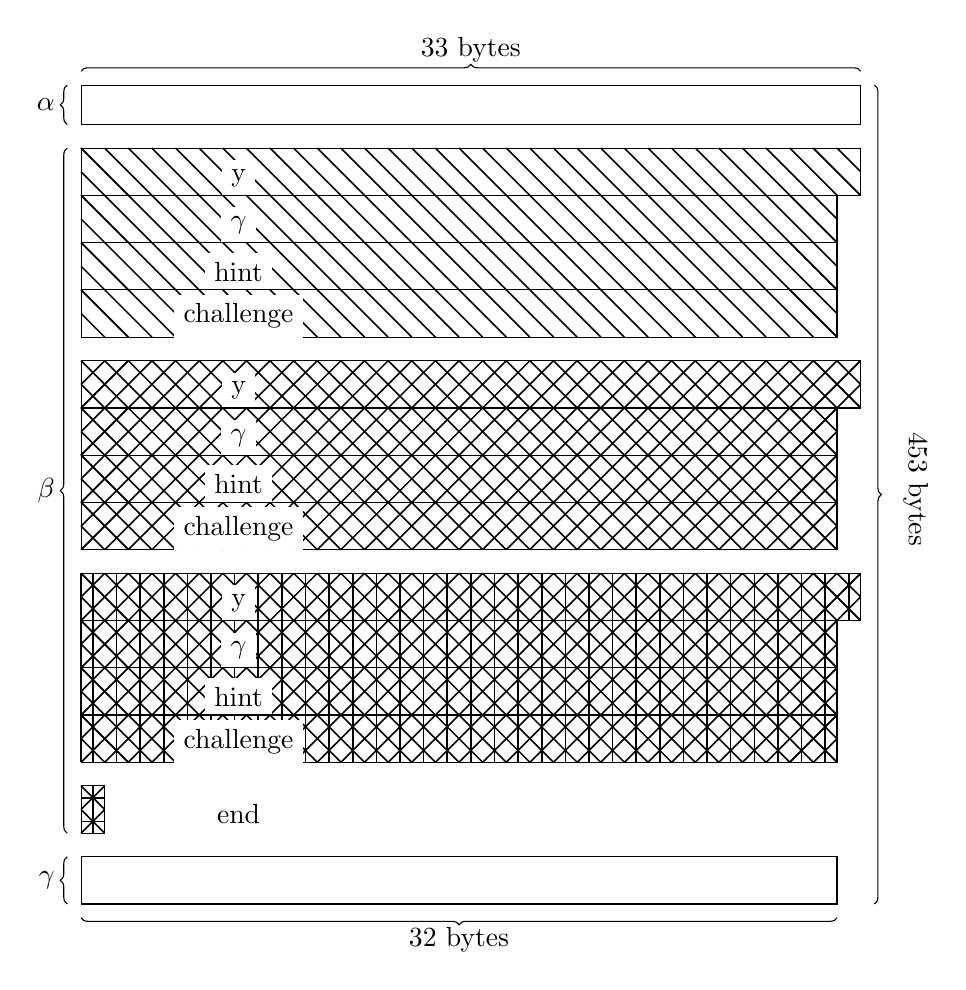
\begin{tikzpicture}
        \def\one{0.3}
        \draw[decoration={brace,raise=5pt},decorate] (0,0.5) -- node[above=5pt] {33 bytes} (33*\one,0.5);
        \draw[decoration={brace,raise=5pt},decorate] (0,0) -- node[left=6pt] {$\alpha$} (0,0.5) ;
        \draw[black] (0,0) rectangle (\one*33,0.5);

        \draw[decoration={brace,raise=5pt},decorate] (0,-9.0) -- node[left=6pt] {$\beta$} (0,-0.3);

        \foreach \name\length\offset\hatching in{y/33/-0.9/1,$\gamma$/32/-1.5/1,hint/32/-2.1/1,challenge/32/-2.7/1,y/33/-3.6/2,$\gamma$/32/-4.2/2,hint/32/-4.8/2,challenge/32/-5.4/2,y/33/-6.3/3,$\gamma$/32/-6.9/3,hint/32/-7.5/3,challenge/32/-8.1/3}{
                \draw (0,\offset) rectangle (\one*\length,\offset+0.6);
                \begin{scope}[shift={(0,\offset)}]
                    \ifnum\length=33
                        \def\a{9.9}
                        \def\diff{9.4}
                    \else
                        \def\a{9.6}
                        \def\diff{9.1}
                    \fi
                    \def\b{0.6}
                    \def\lw{0.2}

                    \foreach \x [count=\i] in{0,0.3,0.6,...,\b}{
                            \draw [line width=\lw mm](\x,0)--(0,\x) (\a-\b+\x,\b)--(\a,\x);
                        }
                    \foreach \x [count=\i] in{0,0.3,0.6,...,\diff}{
                            \draw [line width=\lw mm](\x+\b,0)--(\x,\b); %(\a,\a-\x)--(\a-\x,\a);
                        }

                    \ifnum\hatching>1
                        \foreach \x [count=\i] in{0,0.3,0.6,...,\b}{
                                \draw [line width=\lw mm](0,\x)--(\b-\x,\b) (\a-\b+\x,0)--(\a,\b-\x);
                            }
                        \foreach \x [count=\i] in{0,0.3,0.6,...,\diff}{
                                \draw [line width=\lw mm](\x,0)--(\b+\x,\b); %(\a,\a-\x)--(\a-\x,\a);
                            }
                    \fi

                    \ifnum\hatching>2
                        \foreach \x [count=\i] in{0,0.15,0.45,...,\a}{
                                \draw [line width=\lw mm](\x,0)--(\x,\b);
                            }
                    \fi
                \end{scope}

                \draw (2.0,\offset+0.25) node[fill=white,above=-7.5pt] {\name};

            }

        \draw (0,-8.4) rectangle (\one*1,-9.0);

        \begin{scope}[shift={(0,-9.0)}]
            \def\lw{0.2}

            \draw [line width=\lw mm](0,0)--(0.3,0.3);
            \draw [line width=\lw mm](0,0.3)--(0.3,0.6);

            \draw [line width=\lw mm](0,0.6)--(0.3,0.3);
            \draw [line width=\lw mm](0,0.3)--(0.3,0);

            \draw [line width=\lw mm](0.15,0)--(0.15,0.6);

            \draw [line width=\lw mm](0,0.15)--(0.3,0.15);
            \draw [line width=\lw mm](0,0.45)--(0.3,0.45);

            \draw (2.0,0.25) node[fill=white,above=-7pt] {end};
        \end{scope}

        \draw[decoration={brace,raise=5pt},decorate] (0,-9.9) -- node[left=6pt] {$\gamma$} (0,-9.3);

        \draw (0,-9.3) rectangle (\one*32,-9.9);
        \draw[decoration={brace,mirror,raise=5pt},decorate] (0,-9.9) -- node[below=5pt] {32 bytes} (32*\one,-9.9);

        \draw[decoration={brace,raise=5pt},decorate] (33*\one,0.5) -- node[right=12pt,above=2pt,rotate=-90] {453 bytes} (33*\one,-9.9) ;

    \end{tikzpicture}
    \caption{Sphinx header with PoR}
\end{figure}
